\documentclass[10pt, conference, letterpaper]{IEEEtran}

\usepackage{algorithm}
\usepackage{algorithmicx}
\usepackage{algpseudocode}
\usepackage{amsfonts}
\usepackage{amsmath}
\usepackage{amssymb}
\usepackage{iftex}
% inputenc errors out under xetex/luatex; T1 there restores the classic NFSS
% path so IEEEtran's Times (ptm) resolves with the same metrics as pdflatex.
\ifPDFTeX\usepackage[ansinew]{inputenc}\else\usepackage[T1]{fontenc}\fi
\usepackage{xcolor}
\usepackage{mathtools}
\usepackage{graphicx}
\usepackage{tikz}
\usetikzlibrary{arrows.meta,positioning,calc,fit}
\usepackage{caption}
\usepackage{subcaption}
\usepackage{import}
\usepackage{multirow}
\usepackage{cite}
\usepackage[export]{adjustbox}
\usepackage{breqn}
\usepackage{mathrsfs}
\usepackage{acronym}
%\usepackage[keeplastbox]{flushend}
\usepackage{setspace}
\usepackage{bm}
\usepackage{stackengine}

\usepackage{listings}

\lstset{%
 backgroundcolor=\color[gray]{.85},
 basicstyle=\small\ttfamily,
 breaklines = true,
 keywordstyle=\color{red!75},
 columns=fullflexible,
}%

\lstdefinelanguage{BibTeX}
  {keywords={%
      @article,@book,@collectedbook,@conference,@electronic,@ieeetranbstctl,%
      @inbook,@incollectedbook,@incollection,@injournal,@inproceedings,%
      @manual,@mastersthesis,@misc,@patent,@periodical,@phdthesis,@preamble,%
      @proceedings,@standard,@string,@techreport,@unpublished%
      },
   comment=[l][\itshape]{@comment},
   sensitive=false,
  }

\usepackage{listings}

% listings settings from classicthesis package by
% Andr\'{e} Miede
\lstset{language=[LaTeX]Tex,%C++,
    keywordstyle=\color{RoyalBlue},%\bfseries,
    basicstyle=\small\ttfamily,
    %identifierstyle=\color{NavyBlue},
    commentstyle=\color{Green}\ttfamily,
    stringstyle=\rmfamily,
    numbers=none,%left,%
    numberstyle=\scriptsize,%\tiny
    stepnumber=5,
    numbersep=8pt,
    showstringspaces=false,
    breaklines=true,
    frameround=ftff,
    frame=single
    %frame=L
}

\renewcommand{\thetable}{\arabic{table}}
\renewcommand{\thesubtable}{\alph{subtable}}

\DeclareMathOperator*{\argmin}{arg\,min}
\DeclareMathOperator*{\argmax}{arg\,max}

\def\delequal{\mathrel{\ensurestackMath{\stackon[1pt]{=}{\scriptscriptstyle\Delta}}}}

\graphicspath{{./figures/}}
\setlength{\belowcaptionskip}{0mm}
\setlength{\textfloatsep}{8pt}

\newcommand{\eq}[1]{Eq.~\eqref{#1}}
\newcommand{\fig}[1]{Fig.~\ref{#1}}
\newcommand{\tab}[1]{Tab.~\ref{#1}}
\newcommand{\secref}[1]{Section~\ref{#1}}

\newcommand{\rev}[1]{{\color{blue}#1}}
\newcommand{\red}[1]{{\color{red}#1}}
\newcommand{\mytexttilde}{{\raise.17ex\hbox{$\scriptstyle\mathtt{\sim}$}}}

%\renewcommand{\baselinestretch}{0.98}
% \renewcommand{\bottomfraction}{0.8}
% \setlength{\abovecaptionskip}{0pt}
\setlength{\columnsep}{0.2in}

% \IEEEoverridecommandlockouts\IEEEpubid{\makebox[\columnwidth]{PUT COPYRIGHT NOTICE HERE \hfill} \hspace{\columnsep}\makebox[\columnwidth]{ }} 

\title{Cross-Environment Human Activity Recognition from WiFi CSI:\\ A Controlled Study of Adversarial and Contrastive Training Objectives}

% VERIFY the three addresses before submitting: UniPD student emails often
% carry a disambiguating number (e.g. name.surname.2@studenti.unipd.it).
\author{Filippo Isoni, Filippo Schiabel, Melissa Dedej$^\dag$
\thanks{$^\dag$Department of Information Engineering, University of Padova,
Italy. Emails: filippo.isoni@studenti.unipd.it,
filippo.schiabel@studenti.unipd.it, melissa.dedej@studenti.unipd.it}
}

\IEEEoverridecommandlockouts

\newcounter{remark}[section]
\newenvironment{remark}[1][]{\refstepcounter{remark}\par\medskip
   \textbf{Remark~\thesection.\theremark. #1} \rmfamily}{\medskip}

\begin{document}

% Applies the IEEEtran.bst control entry in biblio.bib (IEEE "et al." rule).
\bstctlcite{IEEEexample:BSTcontrol}

\maketitle

\begin{abstract}
WiFi Channel State Information (CSI) enables device-free human activity
recognition, but a model trained in one room degrades when it is moved to
another, and cross-environment generalization is the main obstacle to
deployment. We ask whether two popular representation-shaping objectives ---
an adversarial domain classifier trained through a gradient reversal layer
(GRL) and a supervised contrastive (SupCon) loss --- improve transfer over
plain cross-entropy (CE), under conditions strict enough for the answer to
mean something: one backbone, one data pipeline, one seed and one
evaluation harness on the SHARP micro-Doppler dataset under a
leave-one-environment-out protocol, with checkpoints selected on validation
only, the test set evaluated exactly once, and differences assessed by a
trace-level paired bootstrap. Neither objective helps, and each fails for its
own measured reason. Our deep residual CE model reaches macro-F1 $0.804$ on
the unseen environment. SupCon loses $7.8$ accuracy points with a bootstrap
interval that excludes zero, and the deficit is in the representation, not the
readout: kNN, nearest-class-mean and a full fine-tune all fail to recover it.
The GRL loses $15.8$ points --- more, but unresolved, its damage falling on a
few traces --- with a $10\times$ larger seed spread, because it has no target:
no domain attribute is linearly readable from the features an adversary reads,
and the dataset's environment incidence leaves the target degenerate. The reference design's shallow--wide network loses $23.5$ points in
the identical recipe. We therefore recommend probing a contrastive encoder
under several readouts, and the nuisance factor for readability, before
investing in either objective.
\end{abstract}

\IEEEkeywords
WiFi sensing, Channel State Information, Human Activity Recognition,
Cross-Environment Generalization, Contrastive Learning, Adversarial Training.
\endIEEEkeywords


% !TEX root = template.tex

\section{Introduction}
\label{sec:introduction}

Wireless sensing turns existing WiFi infrastructure into a device-free
perception system: a moving person perturbs the multipath propagation of the
radio signal, and those perturbations are recorded in the Channel State
Information (CSI) that commodity network cards expose. Human Activity
Recognition (HAR) from CSI needs no wearable, no camera and no cooperation
from the subject, which makes it attractive for assisted living, surveillance
and smart-home applications~\cite{Wang-2019}. The micro-Doppler signature ---
the distribution of reflected power over velocity and time --- is among the
most informative representations derived from CSI, and is our input throughout.

What separates CSI HAR from deployment is not in-distribution accuracy, which
is by now high, but \emph{generalization across environments}: a model trained
in one room entangles the activity with that room's static geometry. The
literature answers with two representation-shaping objectives ---
\emph{adversarial domain invariance}, where a domain classifier behind a
gradient reversal layer (GRL)~\cite{Ganin-2016} pushes the encoder to discard
environment-specific cues, and \emph{supervised contrastive} (SupCon)
learning~\cite{Khosla-2020}, which promises a more transferable embedding
geometry. Both are usually reported on the benchmarks where they helped, each
with its own backbone and protocol; whether they help on a given dataset, and
what must be true of that dataset for them to help at all, is assumed far more
often than it is tested.

We test exactly that, on the SHARP micro-Doppler
dataset~\cite{Meneghello-2023} under a leave-one-environment-out (LOEO)
protocol. Front-end, windowing, backbone, sampler, optimizer, seed and
evaluation harness are held identical, so the training objective is the only
variable; checkpoints are selected on validation alone, the test set is
evaluated exactly once from a frozen row list, and differences are assessed
with a paired bootstrap that treats the recording, not the window, as the
statistical unit. The answer is a controlled negative result, and its value
lies in the explanation: probes on the frozen encoders show that no domain
attribute is linearly readable from the features an adversary would consume,
so on data with this structure the adversarial route could not have worked.
That precondition costs one linear probe on cached features, and we argue it
should be measured before any invariance objective is trained.

\textbf{Contributions.} The key contributions of this report are:
\begin{itemize}
\item A controlled LOEO comparison of CE, CE+GRL and SupCon for
cross-environment CSI HAR under one apparatus and a single-use test protocol;
our CE residual network reaches macro-F1 $0.804$ on the unseen environment and
no variant improves on it.
\item Evidence that neither objective helps: SupCon loses $7.8$ accuracy
points --- the one primary comparison the bootstrap resolves --- and the GRL
$15.8$, with a $10\times$ larger seed spread and most of its damage in the
classifier head rather than in the representation.
\item A measured explanation: no domain attribute is linearly readable from
train features, replicated on five encoders and two rotations, and the
dataset's environment incidence makes this structural rather than accidental.
\item A statistical protocol for small LOEO test sets, under which the
backbone alone is worth $23.5$ accuracy points --- more than any objective we
tested.
\end{itemize}

\secref{sec:related_work} reviews related work,
\secref{sec:processing_architecture} and \secref{sec:model} the pipeline,
signals and splits, \secref{sec:learning_framework} the learning framework,
\secref{sec:results} the results, and \secref{sec:conclusions} concludes.


% !TEX root = template.tex

\section{Related Work}
\label{sec:related_work}

\textbf{WiFi CSI human activity recognition.} Early CSI HAR pipelines fed
hand-crafted amplitude/phase statistics to shallow classifiers; the field then
moved to deep models on time--frequency representations, of which the
micro-Doppler spectrogram is widely used~\cite{Wang-2019}. Our reference point is SHARP~\cite{Meneghello-2023}:
it sanitizes the phase of commodity IEEE~802.11 CSI, reconstructs the channel,
extracts a Doppler representation and classifies with a shallow, wide
convolutional network followed by decision fusion across antennas. SHARP
explicitly targets environment- and person-independence, and its own
evaluation already shows accuracy degrading on unseen rooms --- but it reports
that degradation on a single protocol, without isolating what causes it. We
adopt the cross-environment setting, tighten it into a strict LOEO protocol
with a single-use test session, and reimplement the SHARP network both as a
protocol anchor and as a backbone ablation inside our own recipe, separating
the architecture axis from the objective axis.

\textbf{Domain generalization by adversarial invariance.} The dominant recipe
for making a representation domain-invariant is adversarial: a domain
discriminator is trained on the encoder features while a gradient reversal
layer (GRL)~\cite{Ganin-2016} inverts its gradient into the encoder, so the
encoder is optimized to make the domain \emph{unpredictable} while the task
head still classifies. WiFi sensing pursues the same
invariance~\cite{Wang-2024}, adversarially or by aligning feature
distributions across training environments, on the implicit and rarely tested
precondition that the nuisance factor is present and readable in the features;
when it is not, the adversary reduces to a gradient of noise. A central point
of this report is to \emph{measure} that precondition.

\textbf{Contrastive representation learning.} SupCon~\cite{Khosla-2020}
extends the self-supervised contrastive objective of SimCLR~\cite{Chen-2020} by treating all
same-label samples as positives, and is reported to yield representations more
robust and transferable than cross-entropy ones. The promise is geometric ---
a class-collapsed, well-separated embedding --- but whether that geometry
survives a readout, and whether it transfers across environments, is
empirical: we interrogate it under several readouts and a full fine-tune, so
that a negative result cannot be blamed on one. Other lines pursue
generalization by meta-learning~\cite{Ding-2020} or self-supervised
pre-training~\cite{Yang-2023}; these are out of scope here, since each replaces
backbone and protocol as well as objective --- precisely the confound this
study avoids.


% !TEX root = template.tex

\section{Processing Pipeline}
\label{sec:processing_architecture}

\fig{fig:pipeline} shows the path from a raw CSI recording to an activity
label, from the Doppler front-end to the fusion of the four antenna scores.
Learning acts on the shaded blocks only, and every configuration reuses the
same front-end, windowing, sampler, encoder, fusion rule and harness, so a
difference between two rows is attributable to the training objective and not
to incidental engineering. \textbf{One configuration is deliberately outside
this rule}: C0, the reimplementation of the reference SHARP design, runs on
its own split protocol, five-class label set, backbone and majority-vote
fusion, because it anchors our harness against the prior approach rather than
entering the objective comparison (\secref{sec:res_baseline}); the
architecture axis is isolated instead by an ablation that changes the backbone
\emph{only}.

\begin{figure}[t]
\centering
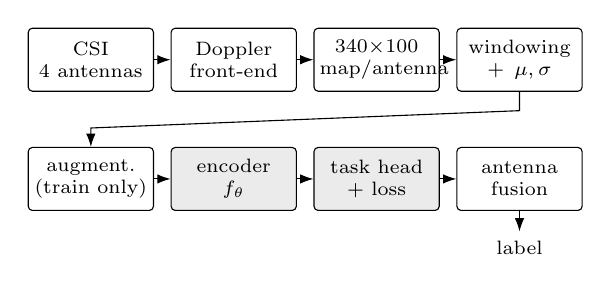
\begin{tikzpicture}[
  font=\scriptsize,
  >={Latex[width=1.2mm]},
  box/.style={draw, rounded corners=1.5pt, align=center, inner sep=2pt,
              minimum height=8mm, text width=14.5mm},
  sh/.style={box, fill=black!8},
  node distance=2.1mm]
\node[box] (csi) {CSI\\4 antennas};
\node[box, right=of csi] (fe) {Doppler\\front-end};
\node[box, right=of fe] (map) {$340{\times}100$\\map/antenna};
\node[box, right=of map] (win) {windowing\\$+\;\mu,\sigma$};
\node[box, below=7mm of csi] (aug) {augment.\\(train only)};
\node[sh, right=of aug] (enc) {encoder\\$f_\theta$};
\node[sh, right=of enc] (head) {task head\\$+$ loss};
\node[box, right=of head] (fus) {antenna\\fusion};
\draw[->] (csi) -- (fe);
\draw[->] (fe) -- (map);
\draw[->] (map) -- (win);
\draw[->] (aug) -- (enc);
\draw[->] (enc) -- (head);
\draw[->] (head) -- (fus);
\draw[->] (win.south) -- ++(0,-2.4mm) -- ($(aug.north)+(0,2.4mm)$) -- (aug.north);
\draw[->] (fus.south) -- ++(0,-2.6mm) node[below, font=\scriptsize] {label};
\end{tikzpicture}
\caption{Processing pipeline. Split and $(\mu,\sigma)$ are frozen before
training; the prediction is the argmax of the softmax averaged over the four
antennas.}
\label{fig:pipeline}
\end{figure}

\section{Signals and Features}
\label{sec:model}

\textbf{Measurement setup.} The SHARP micro-Doppler
dataset~\cite{Meneghello-2023} was collected on a commodity IEEE~802.11 link
with \emph{identical hardware throughout}: domains differ by room, monitor
position, subject, day and line-of-sight condition, never by radio chipset. It
holds three environments (bedroom, living room, laboratory), three subjects
and seven \emph{capture sets} --- one (room, monitor position, subject,
propagation) configuration each --- over twelve campaigns; the unit of
recording is a \emph{trace}, acquired simultaneously on four antennas, and our
inventory counts $101$ traces and $408$ per-antenna streams. Activities carry
the dataset's letter codes: the five-class core is E
(empty room), W (walking), R (running), J (jumping) and L (sitting still), and
the extended set adds C (sit-down and stand-up) plus H and S, two activities
whose letter-to-activity assignment the released package does not document ---
we keep its codes rather than attach a gloss we cannot source.

\textbf{Front-end, windowing and normalization.} The data is distributed as
Doppler traces already produced by the reference front-end (CSI phase
sanitization, channel reconstruction, and a short-time Fourier transform along
the packet axis with hop $T_c \approx 6$\,ms), giving per antenna a map of
reflected power over $100$ velocity bins and time; we consume it as-is, since
keeping the front-end fixed is what isolates the variable under study. Each
map is cut into windows of $340$ time steps $\times$ $100$ velocity bins
($\approx2.0$\,s), with training stride $100$ ($\approx71\%$ overlap) and
validation/test stride $340$ so that evaluation units are \emph{disjoint}: the
primary rotation trains on $\approx69$k (window, antenna) samples and is
tested on $425$ fused windows. Two global scalars $(\mu,\sigma)$, computed on
training windows only, are stored in the frozen split file and reused
unchanged elsewhere. Both axes carry a physical orientation, so flipping
velocity (it inverts the Doppler sign) and reversing time (it maps sit-down
onto stand-up) are forbidden augmentations.

\textbf{Augmentation.} \tab{tab:augment} lists the on-the-fly pipeline,
applied after standardization in a fixed order, masks filled with the
post-standardization mean. The cross-entropy configurations use the moderate
column; the contrastive one draws \emph{two independent views} of each window
with the stronger probabilities of the last column, since SupCon needs views
hard enough for its positives to be informative. Velocity is masked sparingly,
as that axis carries the feature separating walking from running.

\begin{table}[t]
\centering
\caption{Augmentation pipeline, in application order after standardization.
The last two columns give the probability for the cross-entropy profile and
for each of the two contrastive views.}
\label{tab:augment}
\resizebox{\columnwidth}{!}{%
\begin{tabular}{lllcc}
\hline
\textbf{Transform} & \textbf{Axis} & \textbf{Parameters} & \textbf{CE} & \textbf{SupCon view} \\
\hline
Circular shift    & time     & $\pm10$ frames                     & 0.5 & 0.5 \\
Masking           & time     & 1--2 masks, width 5--20            & 0.5 & 0.8 \\
Masking           & velocity & 1--2 masks, width 2--10 bins       & 0.5 & 0.8 \\
Amplitude scaling & ---      & $s \sim \mathcal{U}(0.8,1.2)$      & 0.5 & 0.8 \\
Gaussian noise    & ---      & additive, $\sigma = 0.05$          & --- & 0.5 \\
\hline
\end{tabular}}
\end{table}

\textbf{Splits and rotations.} Two rules are enforced by blocking assertions:
\emph{we split by trace, never by window} --- all windows of a trace, on all
four antennas, fall on one side, since otherwise the static channel leaks and
inflates every metric --- and splits are frozen once as JSON under version
control. The primary rotation holds out the laboratory ($81/9/11$ traces), the
hardest choice available, and a second holds out the living room ($80/6/15$)
for replication; a held-out capture set varies room, monitor position, subject
and day at once, so we speak of held-out \emph{sessions} throughout. Because
the class distribution is very uneven across capture sets, every (capture set,
activity) cell with fewer than four traces has one trace pinned into training;
the price is that no C, E or S trace reaches validation on the primary
rotation, making validation macro-F1 a five-class within-run selection signal
--- common-mode across configurations, and with a per-class effect that
\secref{sec:res_err} measures. A third, leave-the-bedroom-out rotation was
formally rejected before any run: the bedroom holds five of the seven capture
sets, so its training side would be two single-session environments totalling
$26$ traces --- confounding ``the model does not generalize'' with ``the model
had no data'' --- with a two-trace validation split. That same skewed
incidence has a structural consequence (\secref{sec:res_diag}) which the
rejected rotation could only have restated.

\section{Learning Framework}
\label{sec:learning_framework}

\fig{fig:learning} shows how the shared encoder is trained under the three
objectives.

\textbf{Backbones.} C1--C4 share a residual convolutional
encoder~\cite{He-2016} adapted to a $340\times100$ input whose axes are not
interchangeable. A stock ResNet-18 stem would crush the velocity axis to a few
bins; instead the stem (conv $3{\times}3$ and max-pool, both stride $(2,1)$)
and stages 3--4 downsample \emph{time} only, while one isotropic stride
$(2,2)$ in stage 2 halves velocity once, leaving a final map of
$\approx11{\times}50$. The four residual stages are halved in width
($32/64/128/256$ channels) and global average pooling yields the feature
vector, $d_{\mathrm{enc}}=256$; at $4.66$ GFLOPs per window and $2.79$\,M
parameters, the encoder was selected on a throughput and memory gate, not on
accuracy. C0 and the backbone ablation use instead a faithful reimplementation
of the SHARP classifier~\cite{Meneghello-2023}: three parallel shallow
branches concatenated, reduced by a $1{\times}1$ convolution, flattened to
$25\,500$ features and mapped to the classes by one dense layer ---
$\approx1$k convolutional against $\approx204$k dense parameters, a
\emph{near-linear wide} model, the opposite design point.

\textbf{Heads and objectives.} All heads are parametrized on
$d_{\mathrm{enc}}$. The activity head is linear, trained with cross-entropy
and label smoothing $0.1$. The adversarial head is an MLP
($d_{\mathrm{enc}} \to d_{\mathrm{enc}}/2 \to$ 6 capture sets, dropout $0.3$)
behind a gradient reversal layer, giving the C2 objective
\begin{equation}
\mathcal{L} = \mathcal{L}_{\mathrm{act}} + \lambda(p)\,\mathcal{L}_{\mathrm{dom}},
\qquad
\lambda(p) = \frac{2}{1+e^{-10p}} - 1 ,
\label{eq:grl}
\end{equation}
with $p = \min(\mathrm{epoch}/20, 1)$, a ramp fixed in advance so the
adversary reaches full strength independently of when early stopping fires.
The contrastive head is an MLP $d_{\mathrm{enc}} \to d_{\mathrm{enc}} \to 128$
with $\ell_2$-normalized output, trained with the supervised contrastive
loss~\cite{Khosla-2020} at temperature $\tau=0.1$, which pulls together all
views sharing a label against every other view in the batch. C3 trains in two
phases: phase A optimizes it for a fixed horizon of $60$ epochs with no
in-loop selection, checkpointing on a pre-committed grid (epochs $40/50/60$);
phase B freezes the encoder, discards the projection head and fits a linear
probe on cached features, and only the grid checkpoint with the best
validation macro-F1 reaches test. That frozen-probe recipe (Adam, $10^{-3}$,
$\leq30$ epochs, early stopping on the shared metric) is reused for every
probe in this report, so encoders are always compared under one readout.

\begin{figure}[t]
\centering
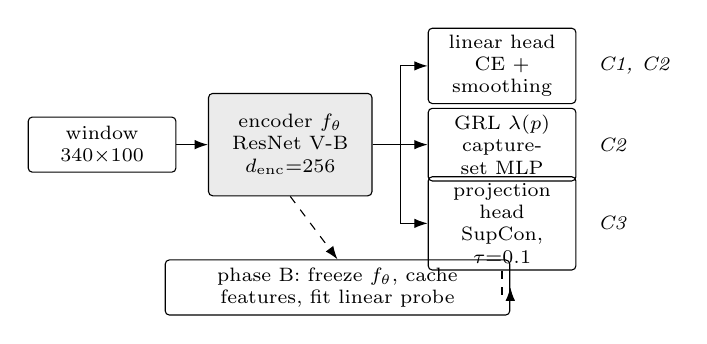
\begin{tikzpicture}[
  font=\scriptsize,
  >={Latex[width=1.2mm]},
  box/.style={draw, rounded corners=1.5pt, align=center, inner sep=2.5pt,
              minimum height=7mm, text width=17mm},
  enc/.style={box, fill=black!8, text width=19mm, minimum height=13mm},
  tag/.style={font=\scriptsize\itshape}]
\node[box] (in) {window\\$340{\times}100$};
\node[enc, right=4mm of in] (e) {encoder $f_\theta$\\ResNet V-B\\$d_{\mathrm{enc}}{=}256$};
\node[box, right=7mm of e, yshift=10mm] (ce) {linear head\\CE $+$ smoothing};
\node[box, right=7mm of e] (grl) {GRL $\lambda(p)$\\capture-set MLP};
\node[box, right=7mm of e, yshift=-10mm] (sc) {projection head\\SupCon, $\tau{=}0.1$};
\node[tag, right=1.5mm of ce.east]  {C1, C2};
\node[tag, right=1.5mm of grl.east] {C2};
\node[tag, right=1.5mm of sc.east]  {C3};
\draw[->] (in) -- (e);
\draw[->] (e.east) -- ++(3.5mm,0) |- (ce.west);
\draw[->] (e.east) -- (grl.west);
\draw[->] (e.east) -- ++(3.5mm,0) |- (sc.west);
\node[box, below=8mm of e, text width=42mm, xshift=6mm] (pb)
  {phase B: freeze $f_\theta$, cache features, fit linear probe};
\draw[->, dashed] (sc.south) -- ++(0,-3mm) -| (pb.east);
\draw[->, dashed] (e.south) -- (pb.north);
\end{tikzpicture}
\caption{Learning framework: one encoder, three objectives --- cross-entropy
(C1), cross-entropy plus a capture-set adversary behind a gradient reversal
layer (C2), and supervised contrastive pre-training read out by a
frozen-encoder linear probe (C3). The dashed path doubles as the diagnostic
instrument: any encoder can be frozen, cached and probed for the activity or
for a domain attribute.}
\label{fig:learning}
\end{figure}

\textbf{Configurations.} The five configurations span a $2{\times}2$ design
over loss family and adversary, plus the anchor: C0 (prior approach), C1 (CE,
our model and internal control), C2 (CE+GRL), C3 (SupCon) and C4 (SupCon+GRL).
C4 was \emph{closed on evidence and never trained}: the diagnostics of
\secref{sec:res_diag} show no readable domain target under either loss family,
so its expected outcome was ``C3 plus noise''. Three pre-registered arms
complete the picture --- C3-ft, a full CE fine-tune from the SupCon encoder;
C1-aug, the amplitude-augmentation arm; and C1-sharplike, the reference
network inside the exact C1 recipe, only the backbone differing.

\textbf{Batching, optimization and reproducibility.} The CE configurations
draw uniform batches of $256$ (window, antenna) samples and optimize an
\emph{unweighted} loss while being selected on macro-F1, a declared asymmetry
kept for comparability with the reference recipe. The contrastive loss is
intra-batch and cannot use uniform batches: a $P{\times}K$ sampler ($P=8$
classes, $K=32$ traces each) draws each class's traces round-robin over the
capture sets where the class exists, making positives ``same activity,
different domain'' by construction, and admits at most one window per trace
per batch (falling back to a $\geq340$-frame offset for classes with fewer
than $K$ traces), since overlapping windows of one recording would reintroduce
the trivial positives that rule exists to remove. Optimization is AdamW
(weight decay $10^{-4}$, peak learning rate $10^{-3}$, cosine decay, $5$
warm-up epochs), mixed precision, gradient clipping at $1.0$, epochs of $400$
fixed steps ($300$ in phase A), at most $40$ epochs, early stopping on fused
validation macro-F1 with patience $10$. Seed $42$ governs initialization,
sampler reseeding and augmentation; two pre-registered seed-$43$ replicates
measure the training-variance floor.

\textbf{Evaluation harness and the single-use test rule.} One shared harness
maps a checkpoint to per-set metric files --- accuracy, macro-F1 (the mean
over classes of the harmonic mean of precision and recall), per-class F1,
confusion matrices and expected calibration error --- always reported with the
number of test traces, since that is the effective sample size. Checkpoints
are selected on validation only and the \emph{test set is evaluated exactly
once}: one session over a frozen, pre-registered row list logged before any
test data is read, so evaluate-then-decide selection is impossible.


% !TEX root = template.tex
% All numbers are final: single §0.7 test session of 2026-07-22
% (reports/final/) + notebook 06 analysis (paired bootstrap N=10000, seed 42;
% tables in report/tables/, summarized in PROJECT.md Part III).

\section{Results}
\label{sec:results}

\textbf{Statistical protocol.} With $11$ test traces the \emph{trace}, not the
window, is the unit of analysis: the windows of one recording share a channel
and are not independent evidence. Differences are assessed by a trace-level
\emph{paired} bootstrap ($N=10^4$) on \emph{accuracy}; macro-F1 is descriptive
only, since just $\sim$2.8\% of resamples contain all eight classes. Bootstrap
and seed variance are never merged, and since $\sim$10 comparisons share the
same traces, C1--C2 and C1--C3 are primary and the rest exploratory.

\subsection{Main results}
\label{sec:res_main}

\tab{tab:test} reports every configuration with its paired accuracy difference
against our model C1. C1 transfers best (macro-F1 $0.804$, seed-stable to
$0.5$ points) and no variant resolves an improvement over it: SupCon falls
$7.8$ and the GRL $15.8$ points below it, while the largest single effect in
the table is not an objective but the backbone, worth $23.5$ points at equal
recipe.

\begin{table}[t]
\centering
\caption{Main results: validation macro-F1 (checkpoint selection), test
macro-F1 and accuracy on the held-out session, and the paired accuracy
difference vs.\ C1 with its 95\% trace-level bootstrap CI ($\ast$ = interval
excludes zero). Top: primary rotation (leave-lab-out, 8 classes, 11 traces).
Bottom: second rotation (15 traces) and the 5-class SHARP anchor on its own
protocol, neither comparable to the top block.}
\label{tab:test}
\resizebox{\columnwidth}{!}{%
\begin{tabular}{llcccl}
\hline
\textbf{Config} & \textbf{Objective} & \textbf{Val F1} & \textbf{Test F1} & \textbf{Test acc} & \textbf{$\Delta$acc vs C1 [95\% CI]} \\
\hline
C1 & CE (our model) & 0.887 & \textbf{0.804} & \textbf{0.805} & --- \\
C1$'$ (s43) & CE, seed 43 & 0.878 & 0.799 & 0.800 & $-0.005$ \\
C2 & CE + GRL & 0.842 & 0.601 & 0.647 & $-0.158\;[-0.323,+0.034]$ \\
C2$'$ (s43) & CE + GRL, s43 & 0.787 & 0.562 & 0.600 & $-0.205$ \\
C3 & SupCon (probe) & 0.819 & 0.729 & 0.727 & $-0.078\;[-0.128,-0.030]^{\ast}$ \\
C3-ft & SupCon + CE ft & 0.818 & 0.706 & 0.720 & $-0.085\;[-0.221,+0.058]$ \\
C1-sharplike & CE, SHARP net & 0.738 & 0.543 & 0.569 & $-0.235\;[-0.399,-0.092]^{\ast}$ \\
\hline
C1-s6out & CE, living-out & 0.776 & 0.684 & 0.743 & (own rotation) \\
C0 & SHARP anchor (5-cls) & 0.892 & 0.605 & 0.612 & (own split) \\
\hline
\end{tabular}}
\end{table}

\subsection{Our model vs.\ the reference design}
\label{sec:res_baseline}

C0 is an \emph{anchor}, not a benchmark reproduction: it follows the published
architecture and majority-vote fusion on the paper's five-class core, but
holds out $20\%$ of the training capture set for early stopping, which the
reference implementation does not. It therefore supports no claim of the form
``we reproduced $X\%$'', only that our apparatus reproduces the
\emph{behaviour} of the prior approach, degrading to macro-F1 $0.605$ over the
held-out capture sets much as the original work reports. Since C0 differs from
our model in protocol, class set, fusion \emph{and} architecture at once, the
like-for-like comparison is the ablation \emph{C1-sharplike}: the reference
network inside the exact C1 recipe, only the backbone changed. It loses $23.5$
accuracy points (test macro-F1 $0.543$ vs.\ $0.804$), CI $[-0.399,-0.092]$ ---
``deep beats near-linear-wide in this recipe'', on one axis only. Its role is
to close the objection that our CE baseline is a strawman, so that the nulls
below are measured against a strong control.

\subsection{Supervised contrastive learning does not transfer better}
\label{sec:res_supcon}

This is the comparison the study was primarily designed to answer, and the
only one the bootstrap resolves. C3's contrastive phase converged cleanly ---
its pre-committed checkpoint grid spans $0.7$ validation points
($0.819/0.815/0.812$ at epochs $40/50/60$), so the selected checkpoint sits on
a plateau --- and on test it lands $7.8$ accuracy points below C1, CI
$[-0.128,-0.030]$.

Since a frozen linear probe could in principle understate a non-linear
representation, we attacked that explanation from four directions.
\emph{Readouts:} on the same frozen validation features C3 scores $0.819$
(linear), $0.805$ (kNN) and $0.718$ (nearest-class mean) in macro-F1 against
C1's $0.884$, $0.856$ and $0.889$; C1 is robust to the readout while C3 loses
under all three, and although kNN beats the class-mean readout on C3 --- so
non-linear structure is genuinely present --- it still does not reach C3's own
linear probe. \emph{Fine-tuning:} unfreezing everything and training with CE
from the SupCon initialization (C3-ft) was pre-registered with the hypothesis
``comparable to C1 within one point'' and falsified it, settling at $0.818$ on
validation --- its own linear-probe ceiling --- and $0.720$ on test.
\emph{Complementarity:} concatenated C1$\oplus$C3 features score $0.868$ on
validation, \emph{below} the same-loss ensemble control C1$\oplus$C1$'$
($0.888$): SupCon is a worse partner than a second CE encoder.
\emph{Geometry:} the left column of \fig{fig:tsne} shows why a linear readout
struggles --- C3's low-motion classes (L, S and the empty room) chain into one
filament instead of three separable blobs --- and the same diagnostic on C3-ft
shows the fine-tune \emph{un-chaining} that geometry, turning the SupCon
encoder back into C1 rather than building on it. Counted honestly this is two families of evidence,
not four instruments: the readouts share cached features and agree partly by
construction, while the fine-tune is a different path and carries the
confirmation. Both point the same way --- the SupCon features are less
informative about the activity, and no head, linear or not, recovers what they
do not encode.

\subsection{The adversary costs accuracy and stability}
\label{sec:res_grl}

C2 loses $15.8$ accuracy points on test. The direction is stable --- it holds
on both seeds (seed-43 gap $20.0$ points) and on validation --- but the
interval $[-0.323,+0.034]$ crosses zero: on $11$ traces even a $16$-point gap
is unresolved. The replicates add a second observation: the
same-configuration spread is
$0.5$ accuracy points for C1 against $4.7$ for C2, so the adversary appears to
cost stability as well as accuracy. A linear probe on C2's \emph{frozen}
features reaches $0.720$ test accuracy, $7$ points above C2's own trained head
($0.647$), against a probe--head gap of $+0.002$ for C1: much of the damage
sits in the classifier head, not in the representation.

\subsection{Why: the adversary has no target}
\label{sec:res_diag}

We answer the natural question --- why an invariance objective fails on a
transfer benchmark --- by probing the \emph{frozen} encoders along the dashed
path of \fig{fig:learning}. On a trace-disjoint inner split of the training
traces we fit linear probes for the activity (positive control) and for every
domain attribute, each against its own majority baseline. The control
saturates ($1.000$ against a $0.197$ baseline) while \emph{every} domain
attribute sits at or below its own: capture set $-0.090$, direct path
$-0.098$, monitor position $-0.086$, and the environment and subject probes
collapse to the constant majority predictor. None of them is linearly readable
from the features, on precisely the data an in-training adversary reads. The
same probes on the C2 and C3 encoders, on all three contrastive checkpoints
and on the second rotation --- five encoders in total --- return the same
verdict, the largest positive deviation anywhere being $+0.015$; the right
column of \fig{fig:tsne} is the geometric counterpart, capture-set colours
uniformly mixed inside every activity cluster.

The implication is structural. A GRL removes domain information its
discriminator can read; here there is nothing to read, so it can only inject
gradient noise --- which is what the training monitors showed (on both seeds
the domain head never left the majority-class floor) and what the test rows
confirm. The root cause is the environment incidence of \secref{sec:model}:
with the bedroom in five capture sets and one set for each other room, any
rotation trains either on a single environment or on one environment plus a
single session, so environment invariance is barely definable on this training
distribution --- which is also why C4 was closed without training, as
evidence-based triage rather than a claim that the GRL is useless in general.
The probe alone shows only that the domain is not \emph{linearly} decodable
from traces the encoder has seen; the structural argument is what generalizes
the verdict.

\begin{figure}[t]
\centering
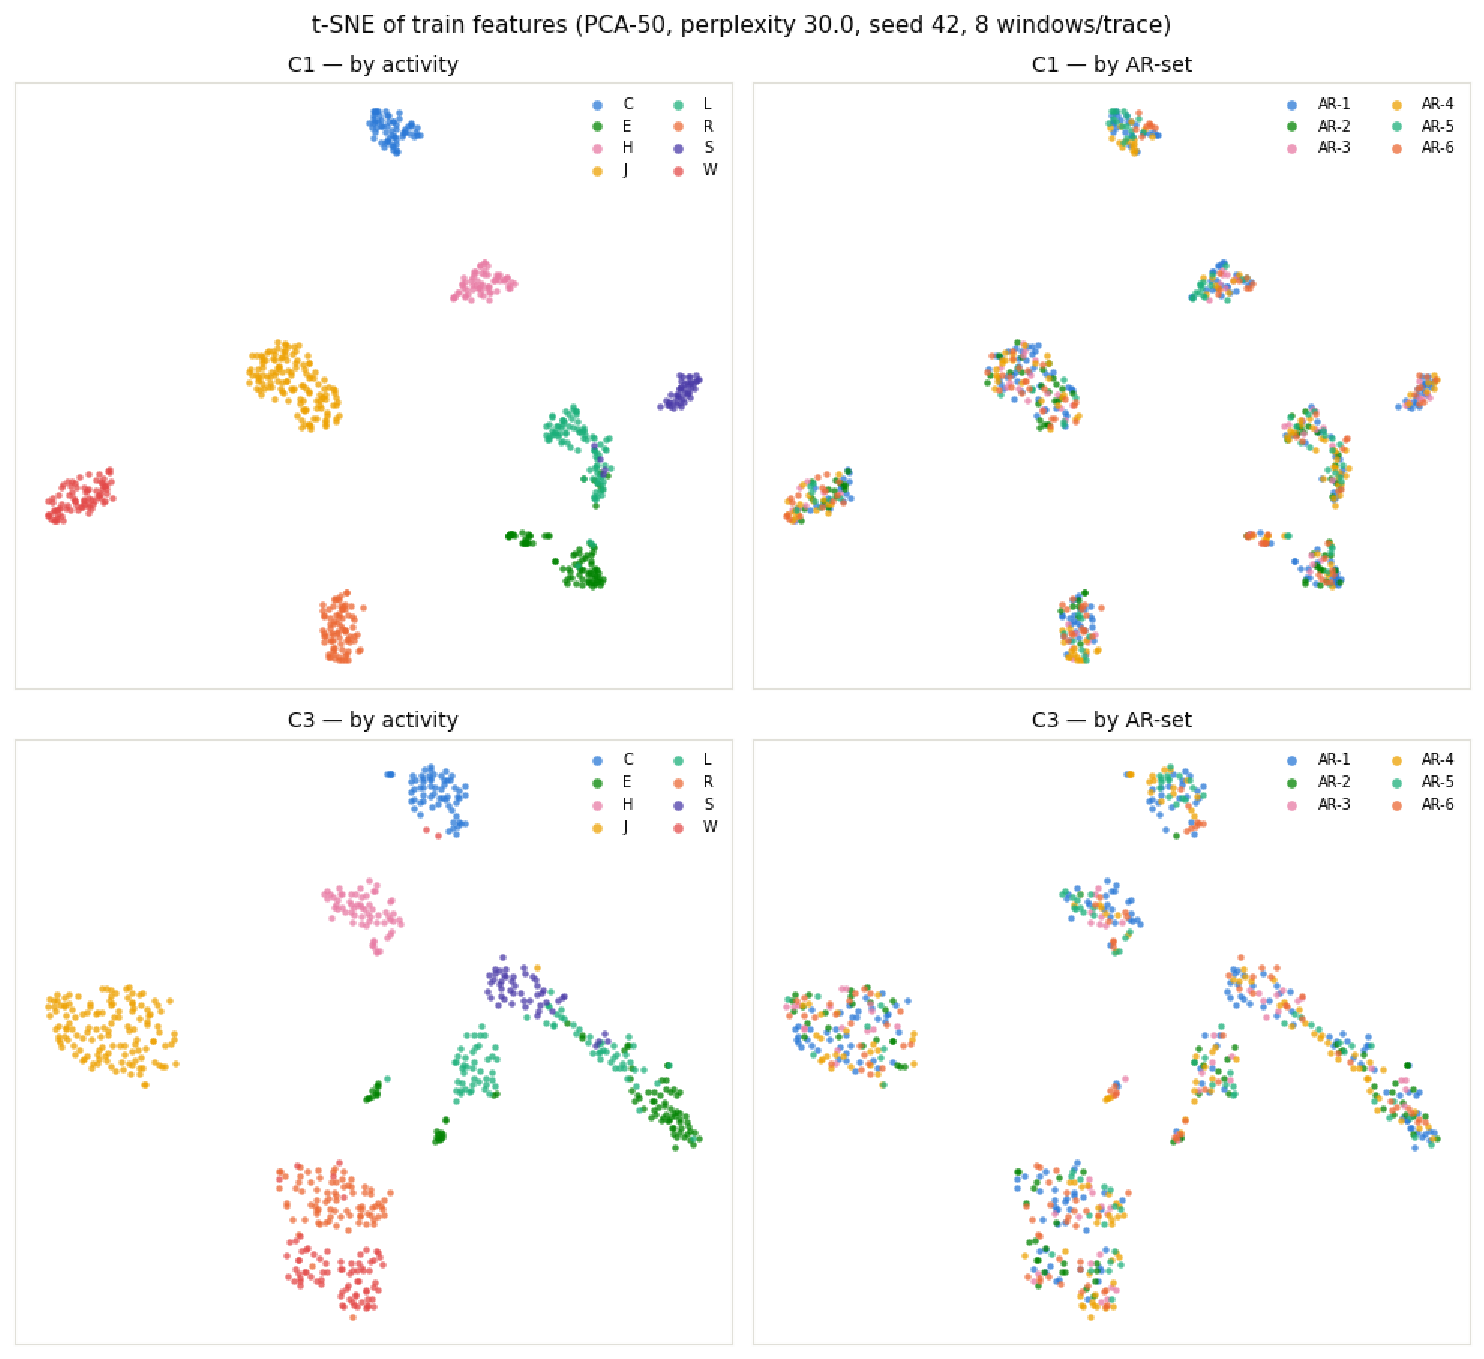
\includegraphics[width=0.88\columnwidth]{embeddings_c1_vs_c3.pdf}
\caption{t-SNE~\cite{vanderMaaten-2008} of train features; top row C1 (CE),
bottom row C3 (SupCon). \emph{Left, by activity:} both form tight clusters,
but C3's L/S/E clusters chain into one filament instead of three separable
blobs --- the geometric counterpart of its lower linear-probe score.
\emph{Right, the same points by capture set:} colours are uniformly mixed
inside every cluster, in both encoders --- no domain sub-structure for an
adversary to remove.}
\label{fig:tsne}
\end{figure}

\subsection{Error structure and limitations}
\label{sec:res_err}

Checkpoint selection was blind to C, E and S, and we had pre-declared the risk
that those classes would underperform; the opposite holds, the val-blind
classes being the \emph{best} ($0.904$ mean F1 against $0.744$), so class
difficulty in the target environment, not selection blindness, drives
per-class error. The errors themselves are
physically sensible (\fig{fig:confusion}): C1 confuses mainly
walking$\leftrightarrow$running and H$\to$J, pairs with adjacent Doppler
signatures, and recognizes the empty room perfectly --- confusions between
physically similar activities, i.e.\ genuine motion features rather than room
artifacts. Calibration
dissociates from accuracy: C1 is systematically \emph{under}confident (ECE
$0.243$, an expected effect of label smoothing) while the GRL model is the
best calibrated ($0.070$) and the least accurate, so any deployment consuming
confidence scores needs temperature scaling.

\textbf{Scope and limitations.} The same session also evaluated two further
pre-registered arms that we do not discuss for lack of space --- test-time
adaptation (AdaBN~\cite{Li-2017}, T3A~\cite{Iwasawa-2021}) and amplitude
augmentation --- neither of which resolved an improvement over C1 (best
$+0.007$, with an interval crossing zero). Beyond those, model selection is
in-domain ($15\%$ of the training traces), so the selected checkpoints may be
sub-optimal out of domain; each held-out set is a single session, so
``environment'' is confounded with subject, monitor position and day; and at
$11$ and $15$ traces a percentile bootstrap separates two or three performance
tiers, not a dozen individually ranked rows.

\begin{figure}[t]
\centering
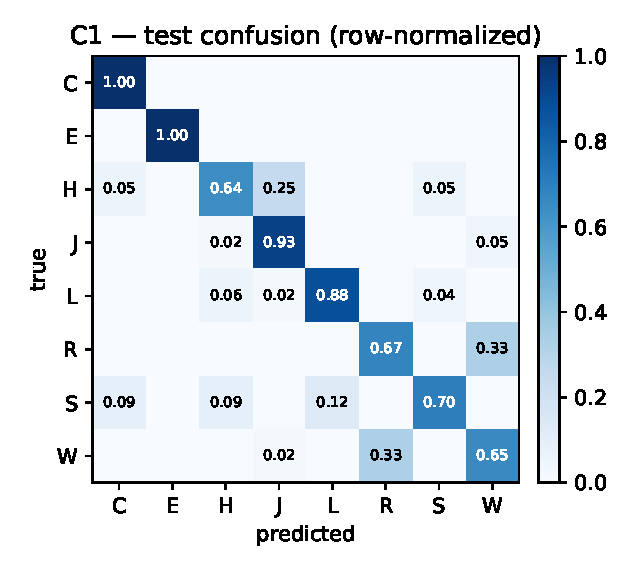
\includegraphics[width=0.44\columnwidth]{confusion_c1_test.pdf}
\caption{Confusion matrix of C1 on the held-out laboratory session
(row-normalized).}
\label{fig:confusion}
\end{figure}


% !TEX root = template.tex

\section{Concluding Remarks}
\label{sec:conclusions}

We evaluated, under one shared apparatus and a single-use test protocol,
whether adversarial (GRL) and contrastive (SupCon) objectives improve
cross-environment WiFi CSI activity recognition over plain cross-entropy. They
do not: SupCon is worse by a bootstrap-resolved margin and the GRL is worse
still and less stable across seeds, while the deep CE model beats the
shallow--wide reference design by $23.5$ accuracy points --- backbone capacity
mattered far more than any invariance objective. The observation we consider most useful is \emph{why} the
objectives fail: frozen-encoder probes show that no domain attribute is
linearly readable from the learned features, so a domain adversary has nothing
to remove --- a precondition that costs one linear probe on cached features to
check, and is worth checking on any dataset whose training split, like this
one, is dominated by a single environment --- a message that goes to benchmark
designers as much as to practitioners.

\subsection{Challenges and Lessons Learned}

Much of this project lay outside the material we had seen: test-time
adaptation, the trace-level paired bootstrap and the frozen-encoder probing
protocol were designed from the literature rather than assembled from known
recipes, and while contrastive learning was familiar in its self-supervised
form, its supervised variant and the gradient reversal layer had to be
implemented and debugged from the original papers. The hardest decisions came
from the data, imbalanced along every axis at once --- environments, capture
sets, subjects and classes --- so that each remedy costs something: pinning
rare cells into training guarantees coverage but empties part of validation,
balancing contrastive batches over capture sets oversamples trace-poor sets,
and a third rotation that looked mandatory on paper had to be rejected for
having $26$ training traces. We also learned to distrust single numbers: the
seed replicates showed a same-configuration swing on the GRL larger than some
cross-configuration gaps, and with $11$ test traces even a $16$-point gap is
unresolved once the honest unit of analysis is the trace. Finally, a caveat we
had declared in advance --- that classes invisible to validation would suffer
--- proved false on test, a reminder that plausible methodological worries
should be measured, not just declared.

\textbf{Future work.} With one held-out session per rotation this is a
transfer study rather than full domain generalization; the natural extension
is a dataset with several well-populated training environments, where our
diagnostic protocol transfers unchanged. Whether \emph{any} training-time
objective can help when the domain factor is unreadable remains open ---
candidates acting on the input, such as physics-informed augmentation, are the
ones unaffected by our structural argument.


\bibliography{biblio}
% IEEEtranBST.bst is the official IEEEtran.bst v1.14, byte-identical, vendored
% under a distinct name: the shipped IEEEtran/ *directory* shadows the plain
% style name and BibTeX aborts trying to open the directory as a file.
\bibliographystyle{IEEEtranBST}

\end{document}


